\documentclass[11pt]{article} %
\usepackage[letterpaper, margin=1in]{geometry}
\usepackage{graphicx,amssymb} %
\usepackage{epstopdf}
\usepackage{amsmath}
\usepackage{fancyhdr}
 
\pagestyle{fancyplain}
\fancyhf{}
\setcounter{page}{1}
\rhead{April 29, 2026}
\lhead{Pace Spring Research Conference 2026}
\cfoot{\thepage}

\begin{document}
% Authors
\title{\ CAMELS: Conversational Agents in Multimodal Embedded Latent Space}


\author{W. Blair, Y. Donegal, K. Jamal, A. Kurup and Faculty Adv Dr. Krishna Bathula,
       \\Seidenberg School of CSIS, Pace University, NY, USA\\       
       \{wb43827n, yd16257n, kj25118n, ak41902n\}@pace.edu\\ 
 }

\date{}

\maketitle

We present CAMELS, a Multimodal Understanding (MU) pipeline and alignment framework designed to enable real-time, naturalistic, Human–Computer Interaction(HCI). Traditional Automatic Speech Recognition (ASR) pipelines rely on converting audio features into textual transcripts as the primary intermediate representation of user utterances. Although this allows text-based LLMs to process user utterances, it introduces a number of critical flaws. First, it discards critical non-textual semantic cues such as tone, speech patterns, and contextual behavioral signals. Secondly, these pipelines rely on components that are not designed to handle streaming interactions. Our approach addresses these limitations by using multi-modal encoding to preserve semantic information as well as a novel temporal chunking strategy to enable real-time comprehension of user interactions.

CAMELS improves training efficiency by leveraging Parameter Efficient Fine Tuning(PEFT) strategies to project multimodal embeddings onto a shared latent space. It further enables online processing of user utterances via temporal chunking and Agentic AI, a stateful agent that tracks and updates conversational context within Latent Representational Space(LRS). CAMELS models conversations in real-time as Hypergraph Neural Networks(HGNNs) that capture higher-order dependencies across speakers, modalities, and temporal segments. These HGNN representations are then used by multi-agent systems to generate naturalistic, context-aware responses across evolving multimodal interactions. We hypothesize that operating directly in LRS will reduce computational overhead sufficiently to enable real-time simulation-based learning exercises. By unifying multimodal signals in a shared latent space, CAMELS provides a practical framework for low-latency, context-aware conversational AI, with planned evaluations targeting multimodal dialogue understanding benchmarks.


\begin{figure}[htb]
\centering
\resizebox{!}{1.8in}{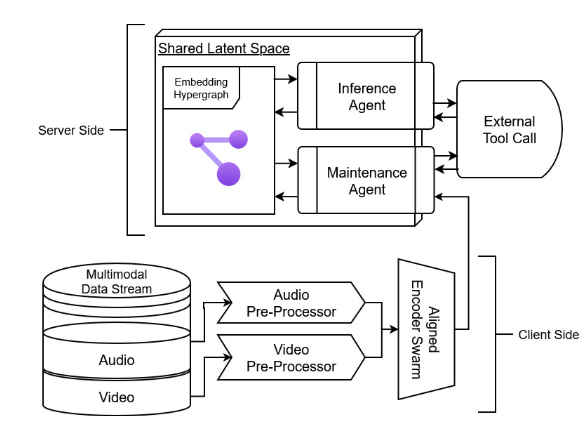
\includegraphics{system_architecture.png}}
\caption{\label{f01} Solution Architecture.}
\end{figure}


\begin{thebibliography}{9}% Replace with at least two references
\bibitem{Li2024Fusion}
W. Li, D. Han, J. Dezert, and Y. Yang,
{\em Multimodal Coordinated Representation Learning Based on Evidence Theory} 2024 27th International Conference on Information Fusion (FUSION), pp. 1–6, Jul. 2024

\bibitem{DuquenneSONAR}
P.A. Duquenne, H. Schwenk, B. Sagot, 
{\em SONAR: Sentence-Level Multimodal and Language-Agnostic Representations} Research - AI at Meta,” ai.meta.com. 

\bibitem{Hao2025CoCoNut}
S. Hao, S. Sukhbaatar, D. Su, X. Li, Z. Hu, J. Weston, and Y. Tian,
{\em Training Large Language Models to Reason in a Continuous Latent Space}
arXiv preprint arXiv:2412.06769v3 [cs.CL], 2025.
\end{thebibliography} 

\section*{Author Biography}
\begin{description}
    \item[Watson Blair] is an MS in Data Science student at Pace University with over seven years of experience as a Full Stack JavaScript engineer.
    \item[Yekaterina Donegal] is an MS in Data Science student at Pace University with a background in Psychology.
    \item[Kiara Jamal] is an MS in Data Science student at Pace University with a background in Software Engineering.
    \item[Arya Kurup] is an MS in Data Science student at Pace University with a background in Artificial Intelligence and Data Science
    
\end{description}


\end{document}
